\chapter{Design}
Systemet er opdelt i tre dele, klienten, serveren og compileren der alle er skrevet i Dart. Databasen var specificeret på forhånd til at være PostgreSQL og skemaet var også defineret. PostgreSQL er en relationel database der har understøttelse for bl.a. JSON.
JSON (Javascript Object Notation) er tekst baseret objekter der gør det muligt nemt at gemme hierarkier og lister, hvilket AdaHeads K/S har udnyttet for at kunne være mere fleksibel over for ændringer i stedet for at skulle redesigne database skemaet hver gang.


\section{Systemoversigt}
\label{sec:adminSystemoversigt}
Det samlet system består af flere maskiner. Den første har Freeswitch og står dermed for at snakke sammen med andre telefonanlæg ude i verden, samt de telefoner som receptionisterne bruger. På den samme maskine er compileren der har adgang til databasen, til når kaldplaner, IVR menuer eller andre dele af den skal konfigureres. Det næste led i kæden af maskiner er der hvor Adaheads K/S Call-Flow-Control program kører, der opdager nye opkald og sørger for at fortælle klienten om det foruden at starte nye opkald, koble opkald sammen og lægge dem på. Det er også her webserveren til det administrative kommer til at køre, selv om det ikke er nødvendigt at de er på samme maskine. Til sidst er der klienten der blot skal have en browser der understøtter HTML5 og CSS3 for så at kunne kommunikere med webserveren.

\begin{figure}[ht!]
\centering
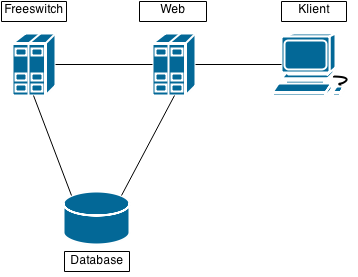
\includegraphics[scale=0.8]{images/systemdiagram.png}
\caption{Diagram over projektets komponenter}
\label{fig:systemdiagram}
\end{figure}

\section{Database}
Datamodellen er lavet så først har man organisationer, som fortæller hvilken virksomhed der skal sendes regninger ud til og hvordan de ønsker dem, samt at den samler flere receptioner. En reception er den kontekst som der bliver ringet ind til. Så i større virksomheder vil der være flere som f.eks. afdelinger eller forskellige butikker rundt omkring i landet og i små virksomheder vil der typisk kun være én reception. En reception består af information om blandt andet hvordan de ønsker håndtering af sælgere, hvad deres CVR numre er og helt lavpraktisk hvad addressen er eller hvad deres åbningstider er og ikke mindst dens kaldplan. 
\begin{figure}[ht!]
\centering
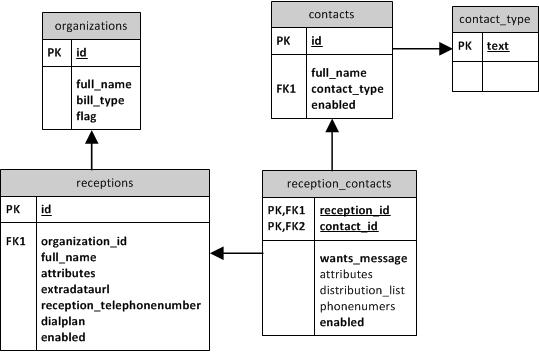
\includegraphics[scale=0.7]{images/ER_Basic.png}
\caption{Udsnit af database skemaet. PK er Primary key. FK er Foreign Key. Tekst i fed skrift er obligatoriske felter.}
\label{fig:erbasic}
\end{figure}

En virksomhed er ikke noget uden deres medarbejder, så til dem er der kontakter som beskriver personen ved deres navn. Det er først i forbindelse med en reception at en kontaktperson har det meste af sin information, som hvad deres telefonnumre og email er, samt information omkring hvad de har af ansvar og hvem deres backup personer er, og den information gemmes i ReceptionContacts tabllen.
Databasen har en flere tabeller end beskrevet her og diagrammet for det fulde database skema kan findes i bilaget.

\section{Server}
Serveren er modelleret op efter MVC arkitekturen, da det passer godt til hvordan en websevrer kan sættes sammen og er godt til at holde de forskellige dele adskildt. Derved har den en række controllere som står for at håndtere forespørgelserne, samt nogle modeller så når dataen kommer ned fra databasen eller fra klienterne, så har man nogle typestærke objekter man kender strukturen af. Serveren har også nogle views der tager sig af at præsenteres modellen i et format der sendes til klienten. 
Serveren er bygget op efter REST principperne, som der kommes mere ind på senere i kapitlet. 

\pagebreak
\section{Brugerfladen}
Brugerfladen er blevet skitseret i samarbejde med AdaHeads K/S og Responsum K/S.
Den er bygget op, så i venstre side har man en menu hvor man kan vælge imellem organisation-, reception-, kontakterperson- og kaldplans-vinduet. Alle 4 vinduer er bygget op omkring 3 søjler for at holde det ensartet.

\subsection{Organisationer}
\begin{figure}[ht!]
\centering
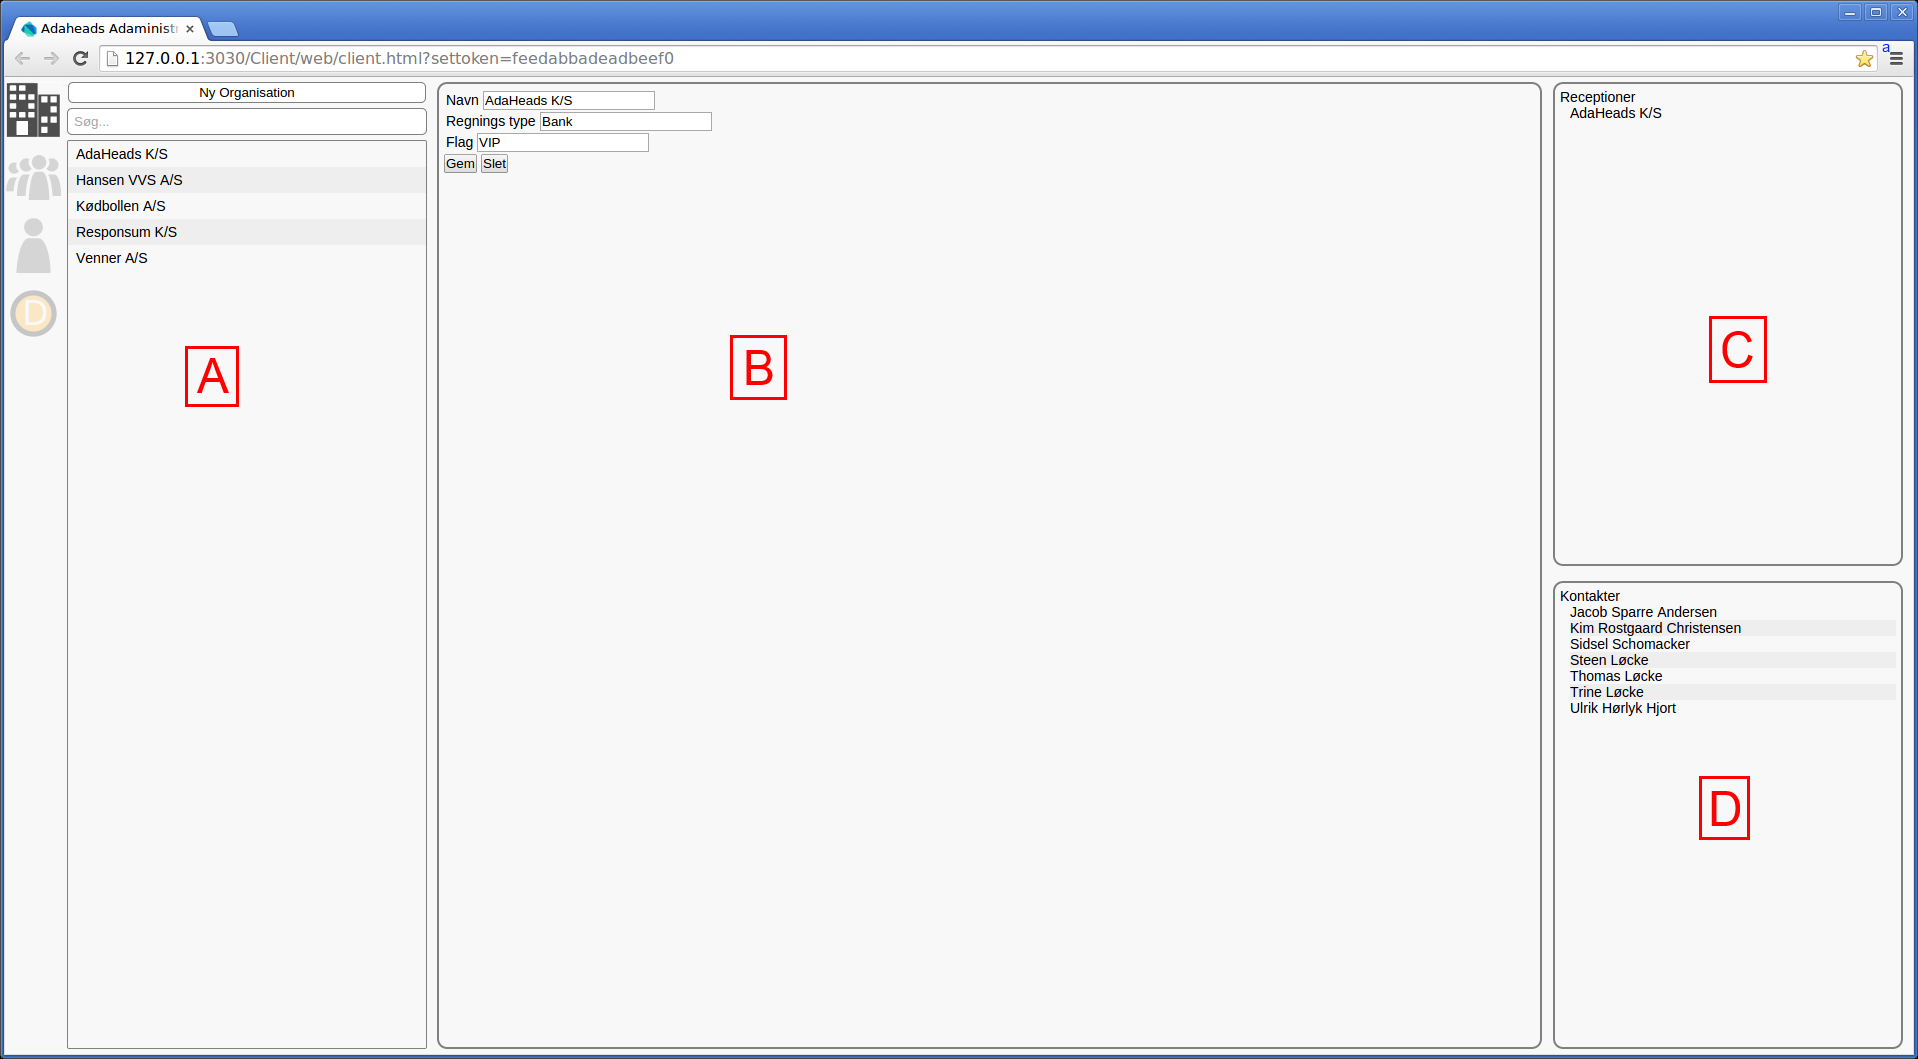
\includegraphics[width=\textwidth]{images/screen_org.png}
\caption{Organisation redigering}
\label{fig:screenorg}
\end{figure}
\begin{enumerate}
	\item[A.] {Set fra toppen mod bunden er der først en knap hvor der kan oprettes nye organisationer, efterfulgt af et søgefelt hvor man kan filtrere på listen af alle organisationer i systemet}
	\item[B.] {Informationen omkring den valgte organisation, samt mulighed for at gemme ændringer og slette organisationen}
	\item[C.] {Liste over receptioner tilknyttet den givende organisation}
	\item[D.] {Liste over samtlige kontakter der er tilknyttet organisationen}
\end{enumerate}

%På organisations vinduet kan man ude i venstre side se en liste af alle organisationer som er tastet ind, og i toppen af den kan man enten skrive i søgefelter som filetere listen %neden under eller trykke for at oprette en ny. 

%I midten kan man indtaste information omkring den pågældende organisation. I den højre søjle er der to lister. Den ene med receptioner og den anden med kontaktpersoner der tilhører den valgte organisation.

\pagebreak
\subsection{Receptioner}
\begin{figure}[ht!]
\centering
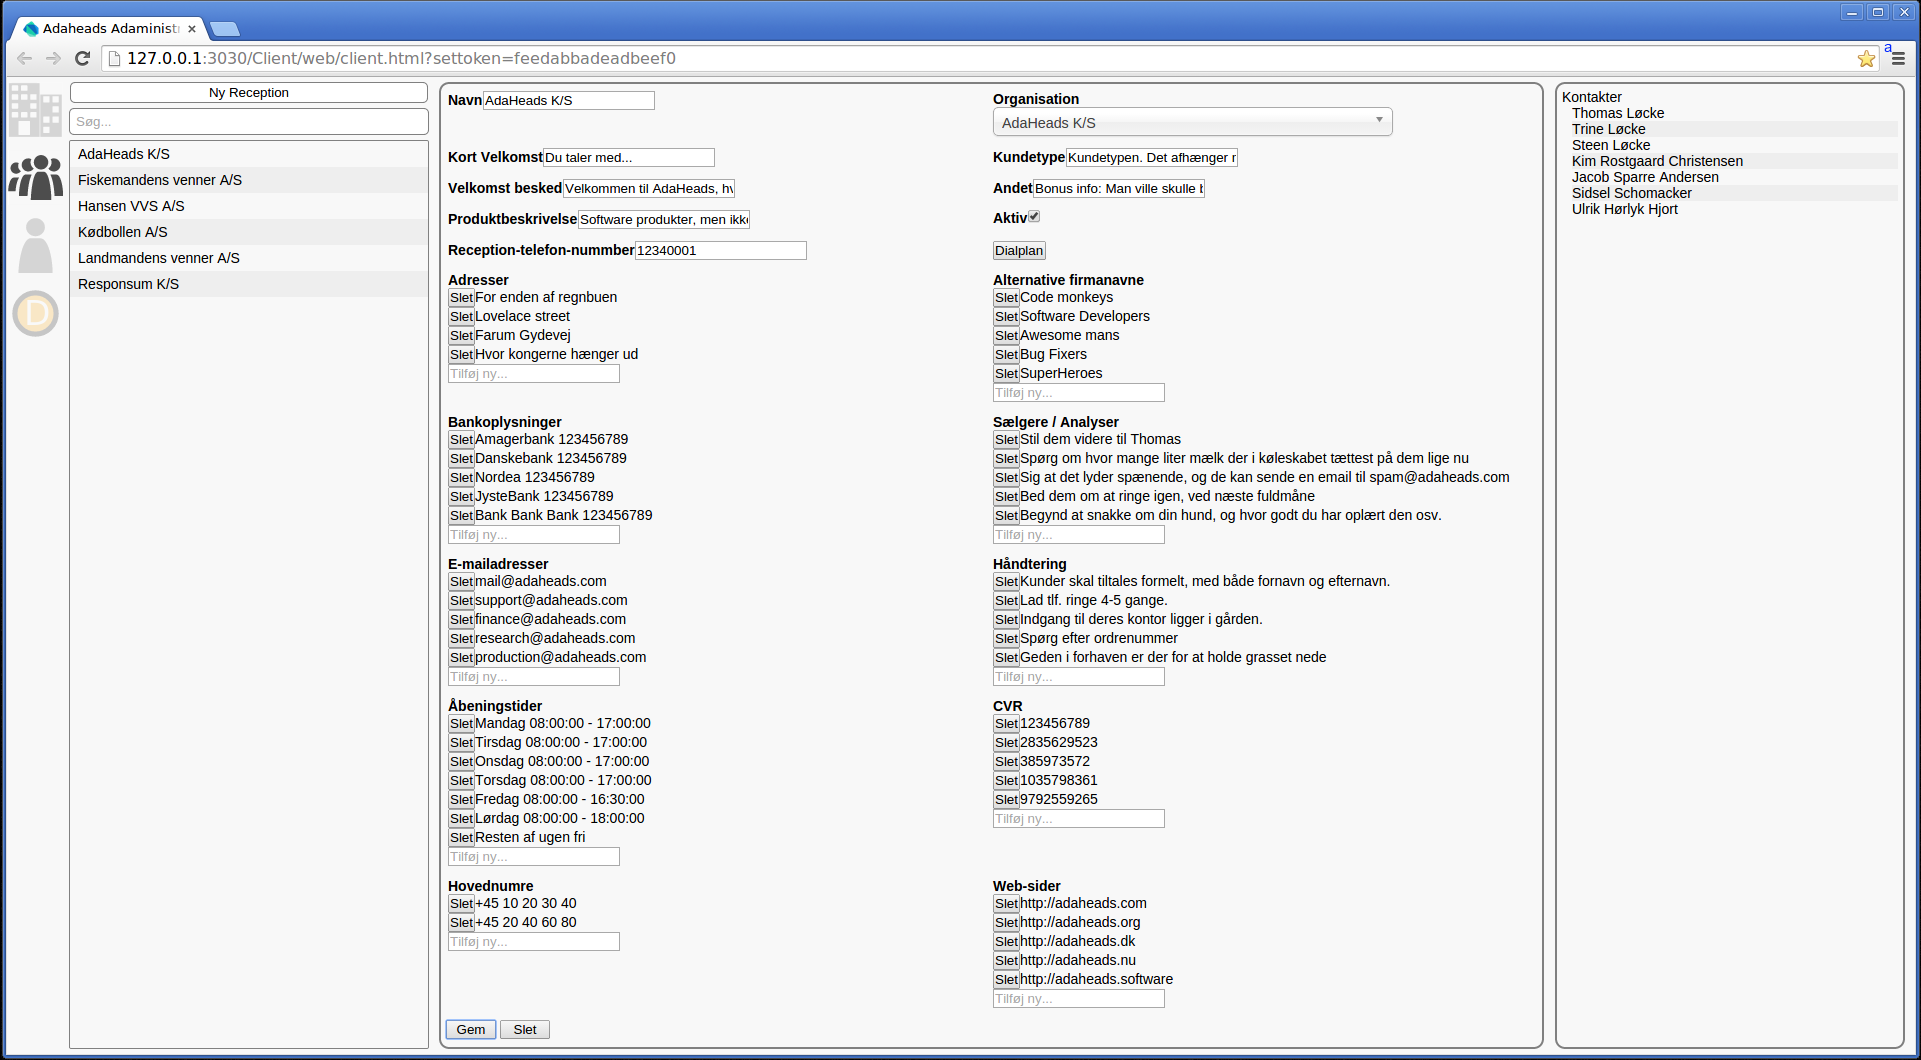
\includegraphics[width=\textwidth]{images/screen_rec.png}
\caption{Reception redigering}
\label{fig:screenrec}
\end{figure}
\begin{enumerate}
	\item[A.] {Set fra toppen mod bunden er der først en knap hvor der kan oprettes nye receptioner, efterfulgt af et søgefelt hvor man kan filtrere på listen af alle receptioner i systemet}
	\item[B.] {Informationen omkring den valgte reception, samt mulighed for at gemme ændringer og slette organisationen. Receptionen indeholder mange lister hvor man kan ved at trække i rækkerne ændre på deres rækkefølge og ved et tryk har man mulighed for at ændre i teksten. I bunden af alle listerne er der et felt hvor der står "Tilføj ny...". Hvis man skriver en tekst i den og afslutter med enter, vil der blive oprette en ny række med den skrevende tekst i}
	\item[C.] {Liste over kontakter tilknyttet den givende reception der ved et tryk på en kontakt kan sende brugeren hen til siden hvor kontakten kan redigeres}
\end{enumerate}

%Reception vinduet er lavet i meget samme stil som organisationvinduet med de 3 søjler. Det har også, hvis vi starter fra toppen i venstre siden, en søjle med en knap hvor der oprettes nye receptioner, et søgefelt for listen neden for, der indeholder alle receptioner. 

%I midten er søjlen med informationen omkring en reception samt to knapper der giver muligheden for enten at gemme de ændringer der er indtastet eller at slette den valgte reception. 

%Til højre er der en søjle med alle kontaktpersoner der har en forbindelse til den valgte receptionen.

\pagebreak
\subsection{Kontaktpersoner}
\begin{figure}[ht!]
\centering
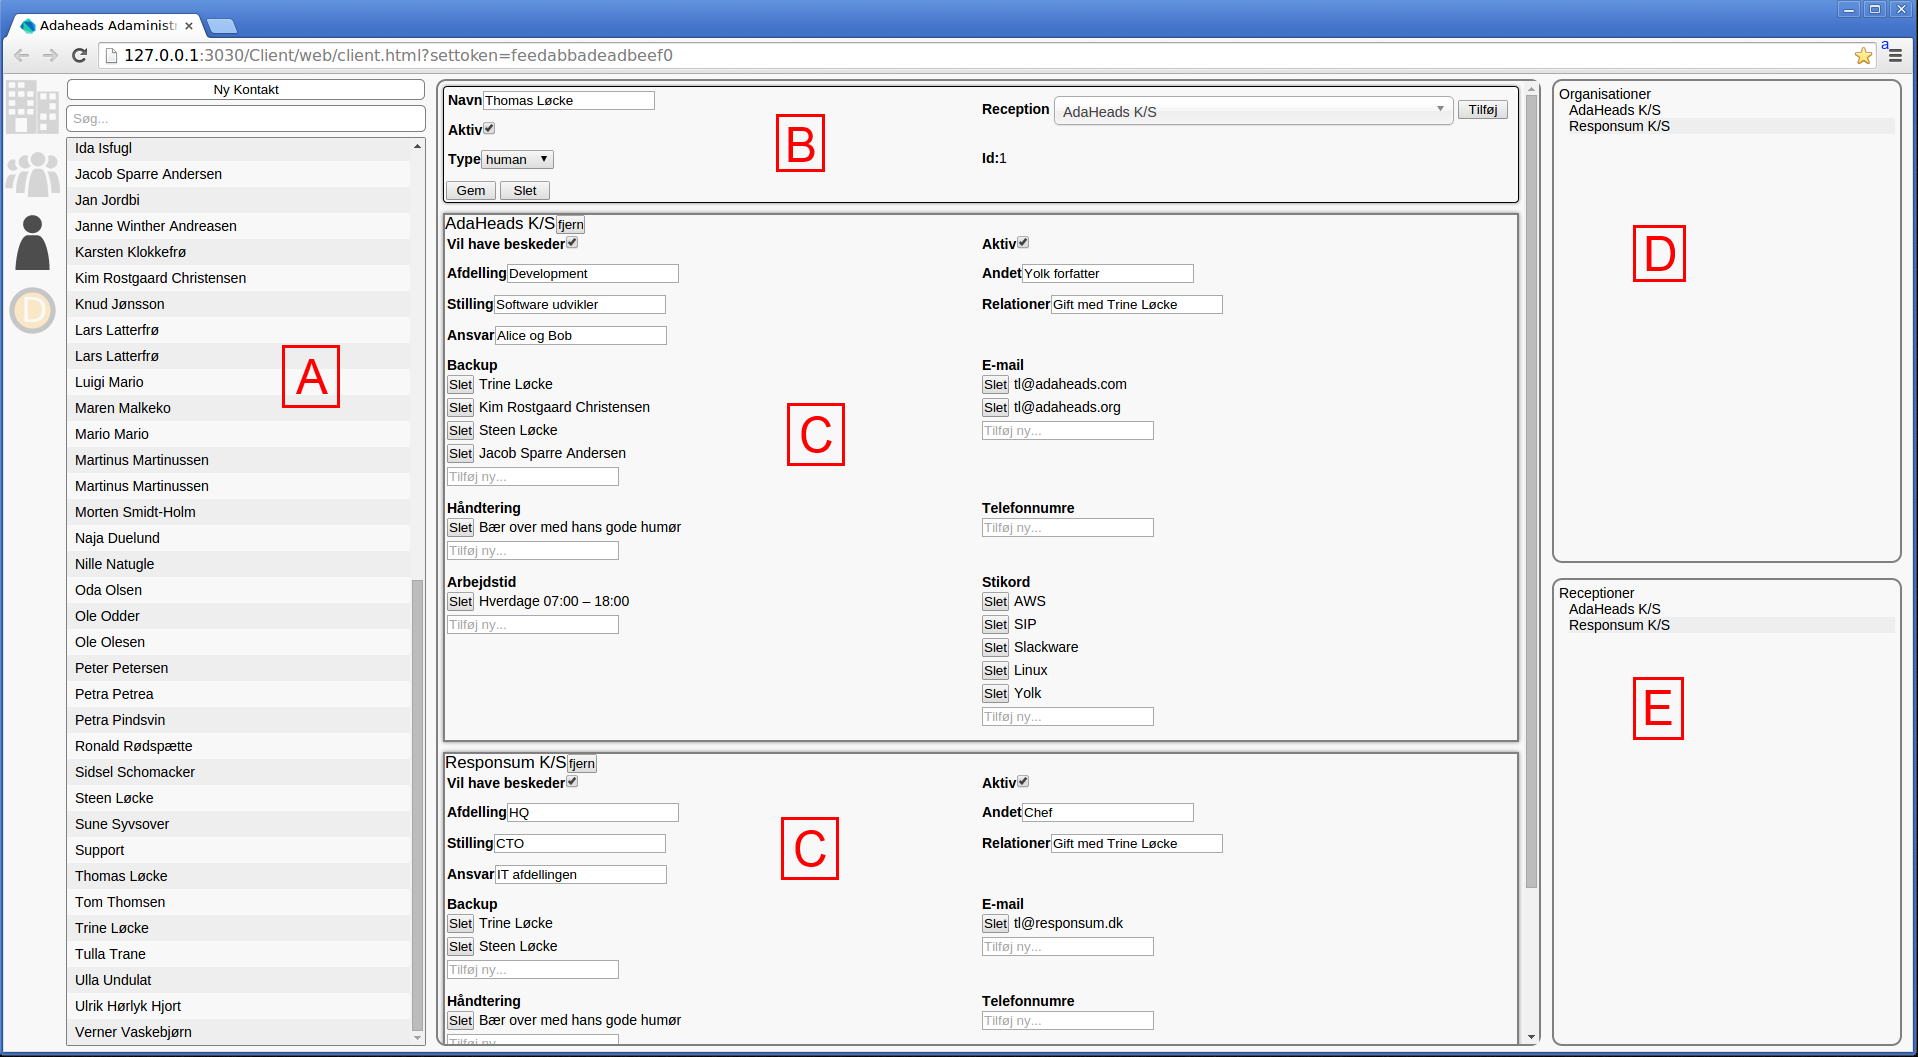
\includegraphics[width=\textwidth]{images/screen_con.png}
\caption{Kontakter redigering}
\label{fig:screencon}
\end{figure}
\begin{enumerate}
	\item[A.] {Set fra toppen mod bunden er der først en knap hvor der kan oprettes nye kontaktpersoner, efterfulgt af et søgefelt hvor man kan filtrere på listen af alle kontakter i systemet}
	\item[B.] {Staminformationen for den valgte kontakt person, samt mulighed for at gemme alle ændringer til kontakt, slette kontakten eller tilføje kontakten til en reception}
	\item[C.] {For hver reception en kontakt er med i, kommer der en boks med den tilknyttede information i}
	\item[D.] {Liste over samtlige organisationer som kontaktpersonen har en tilknytning til}
	\item[E.] {Liste over samtlige receptioner som kontaktpersonen har en tilknytning til}
\end{enumerate}
%I vinduet for kontaktpersoner er der lige som i de forrige to, opret knap, søgefelt og i vinduet her er det en så en liste over kontaktpersoner. I toppen af søjlen i midten er der information omkring en kontaktperson, hvor der er mulighed for at tilknytte en kontakt til en reception. Har en kontaktperson en tilknytning til en reception, så optræder der en boks for hver reception med alt information tilknyttet til den relation. I højre side er der to lister henholdvis hvilke organisationer og receptioner som kontakten optræder i.

\pagebreak
\subsection{Kaldplan}
\begin{figure}[ht!]
\centering
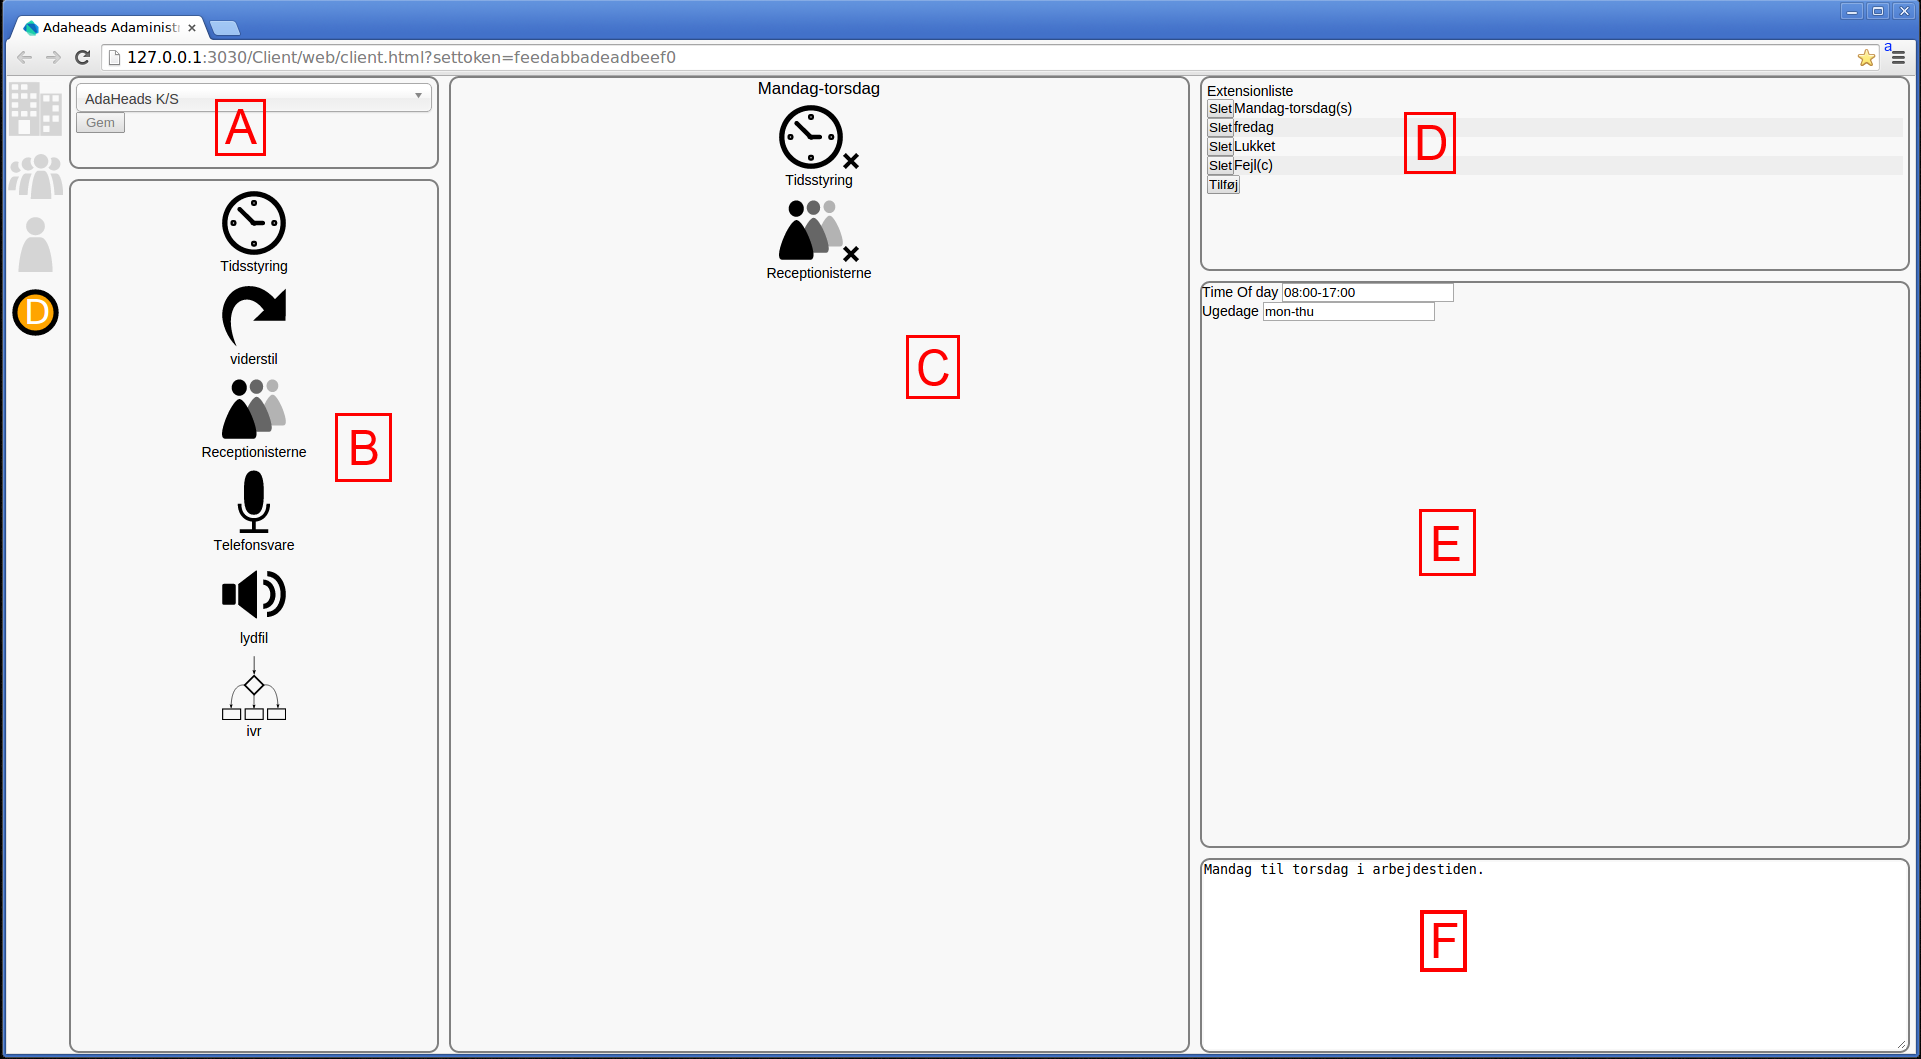
\includegraphics[width=\textwidth]{images/screen_dialplan.png}
\caption{Redigering af kaldplaner}
\label{fig:screendialplan}
\end{figure}
\begin{enumerate}
	\item[A.] {En knap til at gemme ændringer samt en boks som hvis man trykke på den folder den ud til en liste af receptioner med et søgefelt så man kan vælge hvilken receptions kaldplan der skal ændres.}
	\item[B.] {En liste med den betingelser og handlinger man kan sætte ind i en kaldplan}
	\item[C.] {Visning af den valgte extension's betingelser og handlinger}
	\item[D.] {Liste over de extensions der er oprette i kaldplanen}
	\item[E.] {Viser indstillingerne for den valgte kaldplanskomponent, eller extension}
	\item[F.] {Felt til at skrive en kommentar til den valgte komponent, som der kræves fra krav F08}
\end{enumerate}

\pagebreak
\section{Kaldplan-compiler}
Freeswitch er bygget op af en kerne der i sig selv ikke kan bruges som PBX, men med de moduler som følger med kan den bruges til at forbinde IP telefoner eller andre PBX'er, transkode lyd, afspille IVR menuer altså hvad man kræver af de traditionelle PBX og hvis det ikke er nok kan man altid skrive sit eget modul.

Når der kommer et opkald ind i telefonanlægget, skal Freeswitch vide hvordan det skal håndtere opkaldet.
I Freeswitch kan man skrive sin kaldplan i en række af programmeringssprog, men som standart bliver der brugt et modul kaldet mod\_dialplan\_xml og som navnet fortæller så bruger den XML til at beskriver kaldplanen. Der er også den mulighed at lave det, de kalder en outbound socket som fungere ved at man forbinder til deres socket, og der hvor den før hen havde gået ned og læst hvilke applicationer der skulle afvikles, så spørger Freeswitch istedet for på denne forbindelse. 

Adaheads K/S valgte at bruge mod\_dialplan\_xml og derved skrive deres kaldplan i XML. Det giver den fordel at mod\_dialplan\_xml er et gennemprøvet modul og når der skal laves ændringer til en kaldplan så kan man ændre i filerne og bede Freeswitch om at genindlæs dens kaldplaner, hvilket ikke giver nogen nede tid og så er det også en mere stabil løsning. Den mere dynamiske tilgang med en socket er mere fleksibelt, men den statisk udgave ser ud til at kunne det Adaheads kræver af det.

AdaHeads K/S valgte at bruge mod\_dialplan\_xml og dermed skrive deres kaldplaner i XML. Det giver dem en række fordele i forhold til at bruge Freeswitch's outbound socket. 
Først og fremmest skal der ikke udvikles og vedligeholdes et noget nyt program til at kommunikere over deres outbound socket. 
Det næste er at når en dialplan skal ændres kan man blot ændre i XML filerne og bede Freeswitch om at genindlæse dem, hvor derimod at hvis man havde et program skulle man sætte redundante instanser ind, så man kan tillade sig at lukke programmet for at starte den updateret udgave. 
For det tredje så de kriterier som et opkald dirigeres efter vides mange dage på forhånd, så de dynamiske muligheder fra en socket har ikke vist sig nødvendige endnu.

\pagebreak
\section{Mod\_Dialplan\_XML}
\label{sec:moddialplanxml}
En kaldplan er bygget op af en række lag, som det kan ses på figur~\ref{fig:xmldialplan}. 
\begin{figure}[ht!]
\centering
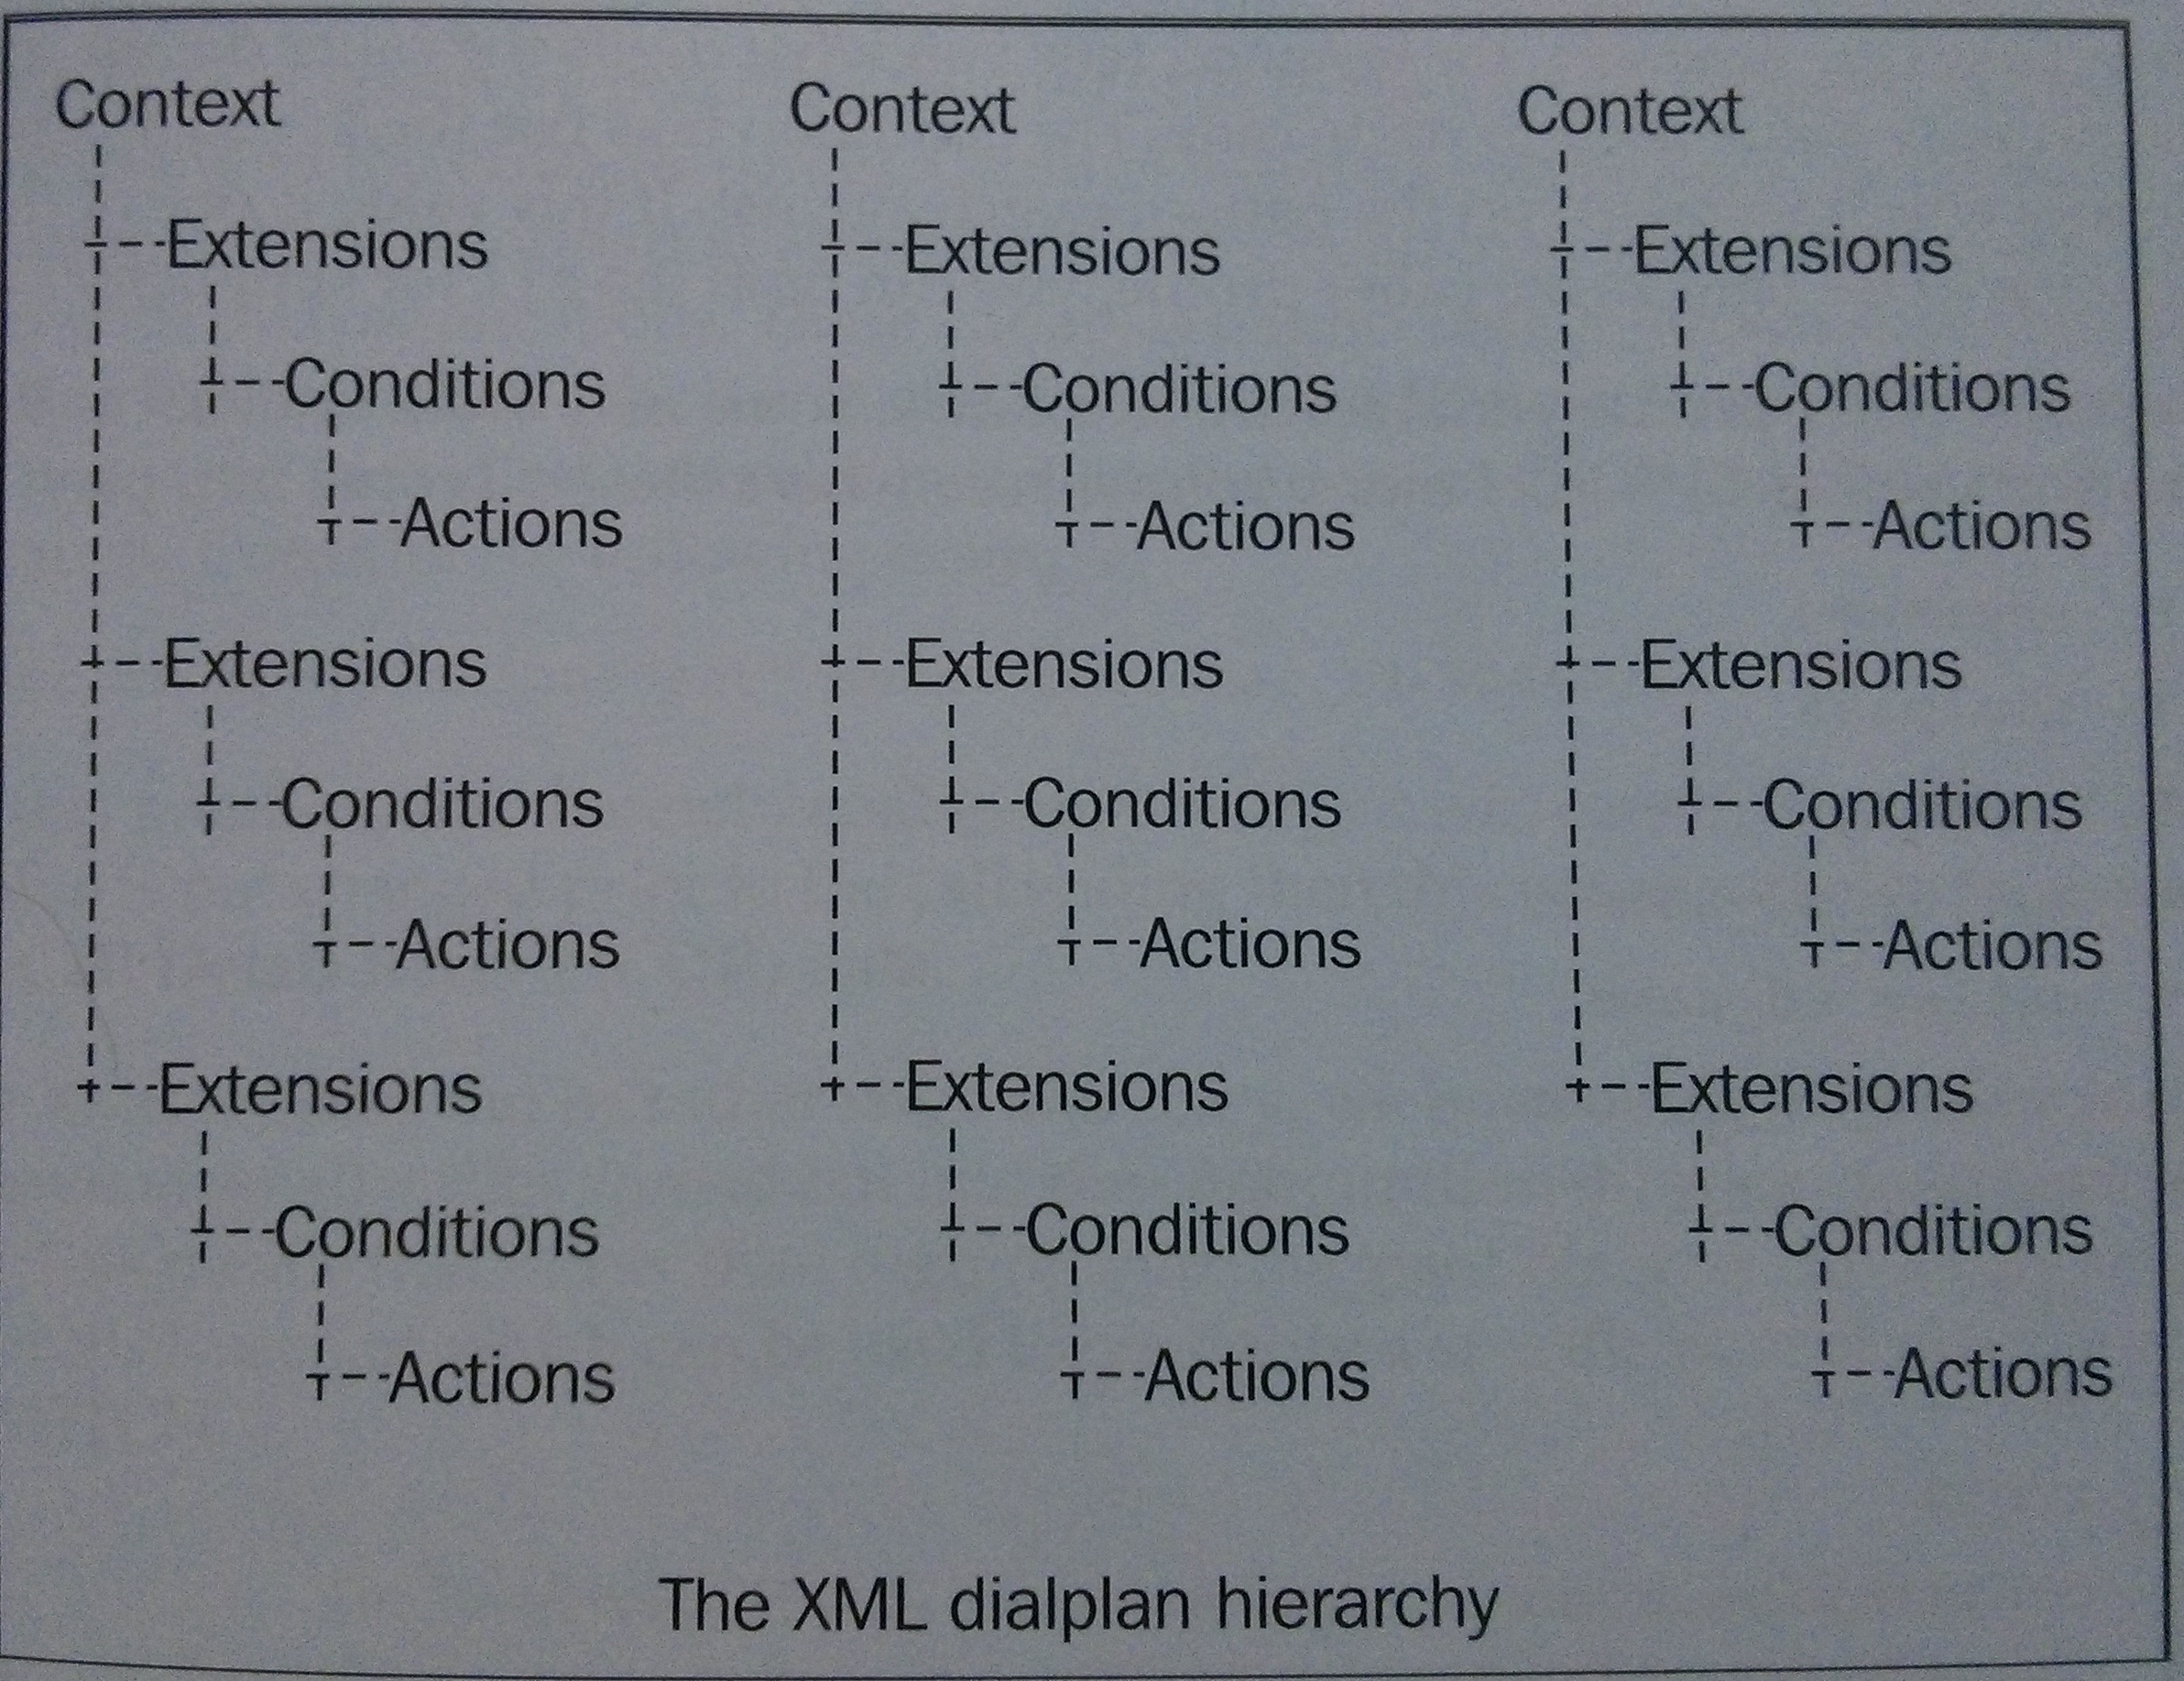
\includegraphics[scale=0.12]{images/dialplanstructure.jpg}
\caption{Strukturen for en XML kaldplan\citep{freeswitch12}}
\label{fig:xmldialplan}
\end{figure}

%\linebreak 
Det først lag er Context. 
En Context er specificeret ved et unikt navn, den kan bestå af flere extensions og en kaldplan kan have flere contexts. Når man registrer en telefon, eller en PBX så konfigureres en context der ringes i. Det har den fordel at man kontrollere hvilke extension som kan ringes ind til fra hver telefonerne og for hver af PBX.

Det næste lag er for extensions. En extension er en gruppering af conditions.
Conditions er som navnet beskriver, de betingelser der skal opfyldes. 
Hvis en condition evaluere til sandt udføres dens actions og hvis ikke så udføres dens anti-actions.
En condition har indbygget funktionalitet til at tjekke på en masse ting omkring tid. F.eks. om det er en bestemt ugedag, eller om klokken er mellem et specificeret interval, hvilket år det er osv. Men udover det kan man kalde andre applikationer og ved hjælp af Regular Expression der bruges til at tjekke svaret, udbygge det til at tjekke hvad som helst. 

Actions og anti-actions er det samme, det eneste der skiller dem ad, er i hvilke omstændighed de bliver udført. Actions er bygget op helt simplet, ved at man specificere et applikationsnavn og dens parameter. For eksempel hvis man ønsker at afspille en lydfil, så sætter man applicationsnavnet til \enquote{playback} og parameteren til stien til filen, så det kunne komme til at se således ud: \linebreak <action application="playback'' data="/home/thomas/welcome.wav"/>

\section{REST}
\label{sec:rest}
Serveren er designet, som nævnt tidligere, i følge principperne bag REST. \linebreak
REST (\textbf{RE}presentational \textbf{S}tate \textbf{T}ransfer) er en web arkitektur der blev opfundet af Roy Fielding i hans ph.d.-afhandling. I den beskriver han at denne arkitektur bygger oven på HTTP og at serveren som klienten snakker med skal være tilstandsløs. Det har en række fordele. Når transportlaget ikke skal holde nogen tilstand, så kan det spare på de fysiske ressourcer og på den måde opnå højere skalerbarhed. Det betyder også at man kan sende forspørgelser parallelt og at der kan køre flere instanser af serveren, og klienten behøver ikke vide hvilken en der snakkes med.
REST er bygget op efter tanken at man arbejder med resourcer, som der kan hentes, oprettes, ændres og slettes igen baseret på et mønster der tager brug af \enquote{method} feltet i HTTP.

Hvis man f.eks. skulle tage udgangspunkt i receptionerne, så kan man hente en bestemt reception på addressen /reception/<id> hvor <id> referere til et tal eller en tekst der kan identificere en bestemt reception og ved bruge method GET, fortæller man at den skal hentes. Spørges der ind til den samme addressen med method valgt til DELETE, så vil den slette receptionen. Lige ledes kan man bruge PUT til at updatere og POST til at oprette nye.
